\chapter{Adaptive Barrier Filtering for Disturbance-Aware Navigation}
\label{ch:contribution}
\section{Adaptive Safety Layer for the Navigation Policy}

The RL policy proposes a nominal action, and the CBF layer filters it before execution. This follows the division between task learning and safety filtering introduced in Section~\ref{ch:rlcbf} and in CBF-RL~\cite{litCBFRL2026}. In our construction, the observer and residual window update during deployment; the policy weights remain unchanged.

\begin{figure}[H]
\centering
\begin{tikzpicture}[font=\small,>=Latex,
 block/.style={draw=navy,rounded corners=3pt,fill=lightblue!55,align=center,minimum height=1.4cm,text width=3.3cm,inner sep=5pt},
 update/.style={block,draw=teal,fill=teal!8},
 flow/.style={->,thick,draw=navy}]
\node[block] (policy) at (0,0) {RL policy\\\footnotesize fixed parameters};
\node[block] (filter) at (4.8,0) {CBF filter\\\footnotesize bounded projection};
\node[block] (robot) at (9.6,0) {Robot\\\footnotesize executed motion};
\node[update] (observer) at (9.6,-3.1) {Disturbance\\observer\\\footnotesize estimate and residual};
\node[update] (risk) at (4.8,-3.1) {Wasserstein--CVaR\\\footnotesize residual buffer and margin};
\draw[flow] (policy) -- node[above] {$u_{B,\mathrm{nom}}$} (filter);
\draw[flow] (filter) -- node[above] {$u_B^\star$} (robot);
\draw[flow] (robot) -- node[right,align=left,font=\footnotesize] {motion and\\last command} (observer);
\draw[flow,teal] (observer) -- (risk);
\draw[flow,teal] (risk) -- node[right,font=\footnotesize] {margin $m_k$} (filter);
\end{tikzpicture}
\caption[Online disturbance adaptation around a frozen policy]{Proposed information flow. Each observer update uses a completed motion interval and its executed command. The estimate and residual history determine the margin $m_k$, while the navigation policy remains fixed.}
\label{fig:contribution_architecture}
\end{figure}

The velocity-command model, clearance normal and CBF condition are defined in Chapter~\ref{ch:system} (Equations~\eqref{eq:contribution_model} and~\eqref{eq:contribution_normal}).

\section{EMA Estimation and Rolling Residual Window}

\subsection{Disturbance Estimate Update}

At update $k$, the completed motion interval provides a displacement and its previously executed world-frame command $u^\star_{W,k-1}$. With sampling interval $\Delta t$, the observer computes
\begin{align}
 d^{\mathrm{raw}}_{k-1}
 &=\frac{p_k-p_{k-1}}{\Delta t}-u^\star_{W,k-1},
 \label{eq:contribution_raw}\\
 r_{k-1}&=d^{\mathrm{raw}}_{k-1}-\hat d_{k-1},
 \label{eq:contribution_residual}\\
 \hat d_k&=\hat d_{k-1}+\ell r_{k-1},\qquad 0<\ell<1.
 \label{eq:contribution_observer}
\end{align}
This EMA-inspired observer tracks recent disturbance while smoothing the raw measurements. It uses the disturbance-estimation principle discussed in Section~\ref{ch:disturbanceprior}~\cite{litDOB1987,litDOB2015}. A larger gain follows changes more quickly; a smaller gain produces a smoother estimate.

Reconstruction uses the action actually executed after filtering, so the filter's correction is not mistaken for an external disturbance. The residual is computed against the previous estimate, before the EMA update. It therefore records the prediction error present during that completed interval.

The raw quantity is an interval-average motion mismatch. Position noise and imperfect command tracking can contribute to it alongside wind. We use the residuals of this observable mismatch directly, without fitting a separate aerodynamic model.

\subsection{Recent Prediction Error Window}

The rolling window keeps at most $M$ residual vectors. For $k\geq1$, its index set and empirical distribution are
\begin{equation}
\begin{aligned}
 \mathcal I_k&=\{\max(0,k-M),\ldots,k-1\},\qquad N_k=|\mathcal I_k|,\\
 \widehat P_k&=\frac1{N_k}\sum_{i\in\mathcal I_k}\delta_{r_i}.
\end{aligned}
\label{eq:contribution_empirical}
\end{equation}
Once the window is full, each new residual replaces the oldest one. The empirical distribution therefore moves with the recent operating conditions instead of retaining the entire mission history.

A shorter window emphasizes responsiveness; a longer window retains more information about infrequent errors. The window has a fixed capacity but advances in time. It is this renewal of its contents that supplies the online adaptation.

No Gaussian density or mixture model is fitted. The sample cloud can be asymmetric or multimodal, and the original residual vectors remain available for projection onto the current obstacle direction. This makes the temporal observations directly usable by the safety layer.

\section{Wasserstein Neighborhood of the Residual Distribution}

\subsection{Transport Distance}

A new residual need not coincide with any point in the current empirical distribution. Wasserstein distance gives a geometric meaning to this displacement. For distributions with finite first moments, the 1-Wasserstein distance with Euclidean ground cost is
\begin{equation}
 W_1(P,Q)=\inf_{\Gamma\in\Pi(P,Q)}
       \int\norm{r-s}_2\,d\Gamma(r,s),
 \label{eq:contribution_wasserstein}
\end{equation}
where $\Pi(P,Q)$ contains the couplings with marginals $P$ and $Q$. It measures the least average distance needed to transport one probability distribution into the other.

The support-based examples in the Wasserstein GAN paper provide useful intuition~\cite{thArjovsky2017}: a distribution can move a small distance without overlapping its original support. Wasserstein distance reflects that movement. In contrast, $D_{\mathrm{KL}}(P\Vert Q)$ is infinite whenever $P$ gives positive probability to a set assigned zero probability by $Q$.

\begin{figure}[htbp]
\centering
\begin{tikzpicture}[font=\small,>=Latex]
\draw[->,navy] (-.5,0) -- (10.5,0) node[right] {$r$};
\foreach \x in {1,4,7}{
 \draw[navy,very thick] (\x,0) -- (\x,1.05);
 \fill[navy] (\x,1.05) circle (3pt);
 \draw[teal,very thick] (\x+1,0) -- (\x+1,1.85);
 \fill[teal] (\x+1,1.85) circle (3pt);
 \draw[->,thick,orange!80!black] (\x,2.35) -- (\x+1,2.35);
}
\node[anchor=west,navy] at (0,3.2) {Empirical masses};
\node[anchor=west,teal] at (5.6,3.2) {Shifted masses};
\node[align=center] at (4.5,-.8) {Same weights, disjoint locations, displacement $\Delta\ne0$};
\node[align=center,fill=lightblue!50,rounded corners,inner sep=8pt] at (4.5,-1.75)
 {$D_{\mathrm{KL}}(P\Vert Q)=\infty$
 \qquad $W_1(P,Q)=|\Delta|$};
\end{tikzpicture}
\caption[Transport distance for displaced empirical samples]{A one-dimensional illustration of the support issue. Three equally weighted point masses are translated by the same nonzero displacement to disjoint locations. Vertical offsets distinguish the two sets; they do not represent different probability weights. Wasserstein distance records the displacement, while KL divergence is infinite. The example follows the support-based intuition of Arjovsky et al.~\cite{thArjovsky2017}.}
\label{fig:contribution_support}
\end{figure}

\FloatBarrier
\subsection{Uncertainty in the Observed Distribution}

For our residual window, construct
\begin{equation}
 \mathcal P_k(\rho)=
 \{Q\in\mathcal P_1(\R^3):W_1(Q,\widehat P_k)\leq\rho\},
 \label{eq:contribution_ball}
\end{equation}
where $\mathcal P_1$ denotes distributions with finite first moments. We write the radius as $\rho$, distinguishing it from the residual vectors $r_i$. The center $\widehat P_k$ changes with the window; the radius sets the allowed disagreement with the observed residual distribution.

\begin{figure}[htbp]
\centering
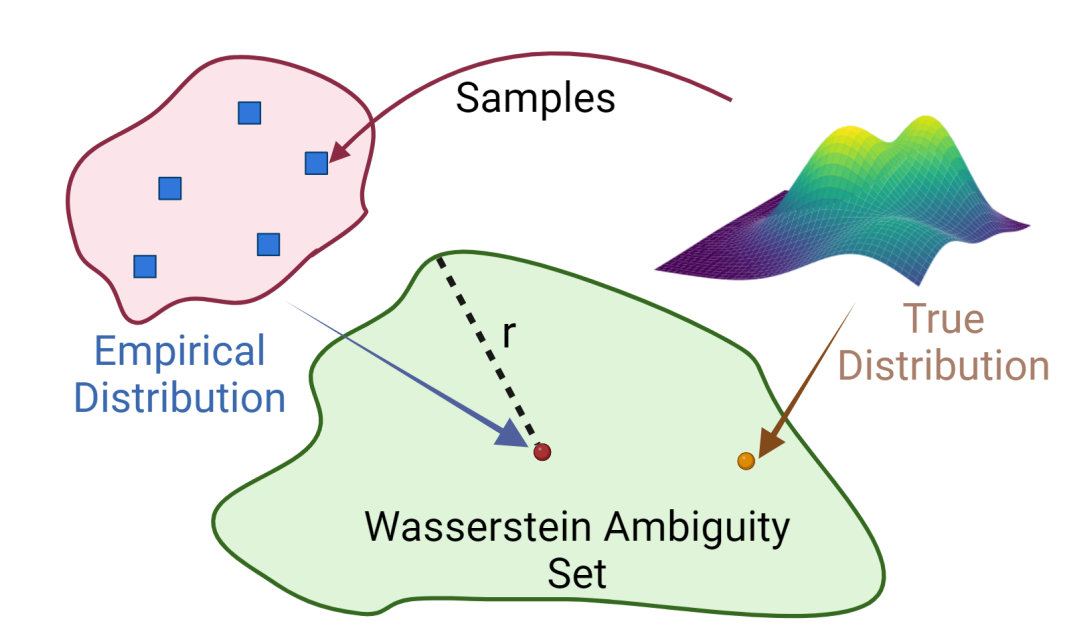
\includegraphics[width=.97\textwidth]{figures/long_wasserstein_ambiguity.png}
\caption[Wasserstein ambiguity set]{Wasserstein ambiguity set, from Long et al.~\cite{long2024sensor}, Fig.~3. The radius labeled $r$ corresponds to $\rho$ here. Each point in the lower schematic represents a distribution, not a residual sample. The true distribution is shown inside the neighborhood as an illustration of the intended coverage.}
\label{fig:contribution_ball}
\end{figure}

This construction admits previously unseen residual values without choosing a parametric density. It also connects to tractable CVaR bounds for affine directional losses~\cite{thEsfahani2018,long2024sensor}. The distributional allowance can consequently be evaluated before the final command projection.

\FloatBarrier
\section{Residual-Based Safety Margin}

\subsection{Adverse Tail of the Residuals}

At the current update, the clearance-reducing residual is $z_k(r)=-n_k^\top r$. Positive values describe unmodeled motion toward the obstacle. Every vector in the window is projected onto the current normal, so the risk calculation follows the present geometry.

Conditional value-at-risk (CVaR) summarizes the adverse tail of these projected residuals. With upper-tail probability $\epsilon\in(0,1)$, the empirical calculation is
\begin{equation}
 \widehat{\cvar}_{\epsilon,k}(z_k)=
 \min_{\eta\in\R}\left\{
 \eta+\frac1{\epsilon N_k}
 \sum_{i\in\mathcal I_k}(z_k(r_i)-\eta)_+
 \right\}.
 \label{eq:contribution_cvar}
\end{equation}
The threshold $\eta$ separates the adverse tail. The positive-part term measures exceedances above it. This definition applies directly to empirical samples, including repeated values and fractional sample mass at the threshold~\cite{thRockafellar2002}.

\begin{figure}[htbp]
\centering
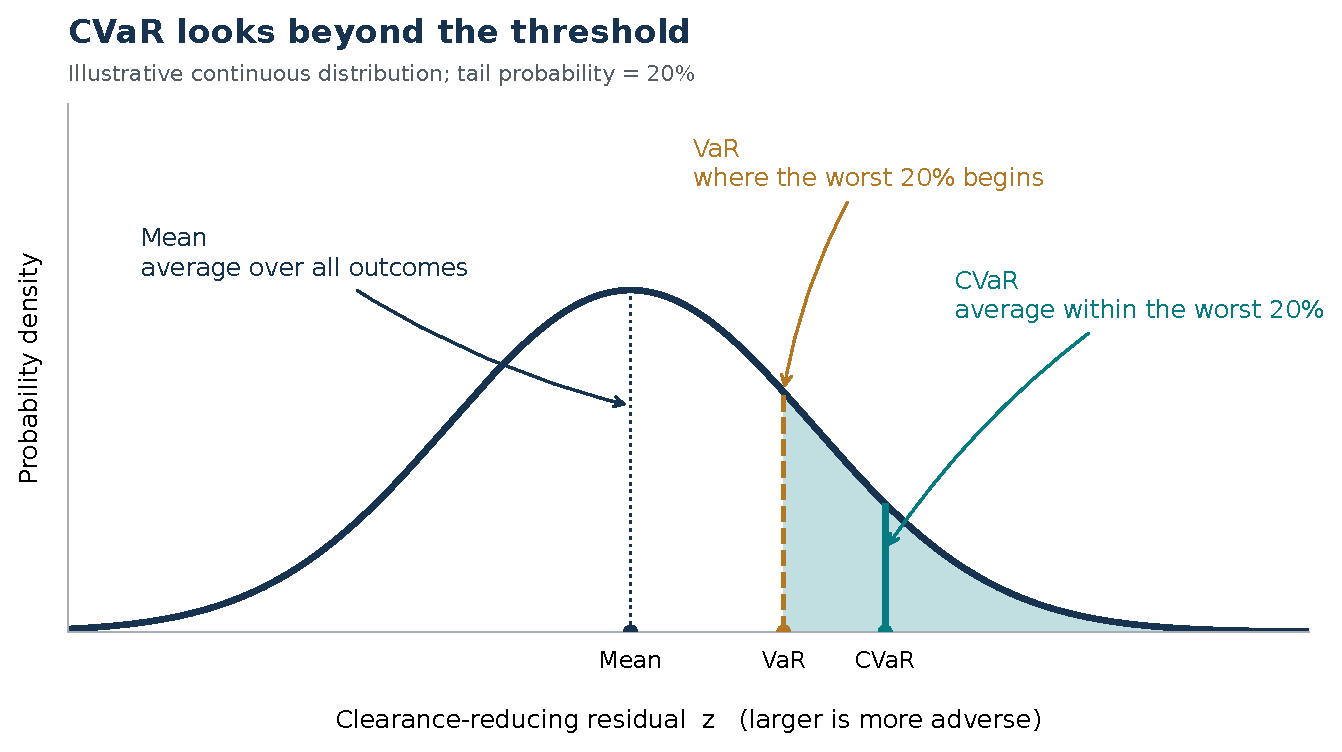
\includegraphics[width=\textwidth]{figures/cvar_tail_explanation.pdf}
\caption[Understanding CVaR through the adverse tail]{The mean averages all outcomes. VaR locates the beginning of the adverse tail; CVaR measures the average loss within that tail for this continuous illustration. The shaded region contains the worst 20\% of outcomes, chosen only to make the concept visible. The density is an explanatory example, not a fitted residual model or experimental result. For an empirical distribution, Equation~\eqref{eq:contribution_cvar} handles the possible fractional mass at the threshold~\cite{thRockafellar2002}.}
\label{fig:contribution_tail}
\end{figure}

\FloatBarrier
\subsection{Estimation and Distributional Uncertainty}

The observer contributes the estimated adverse component $-n_k^\top\hat d_k$. CVaR describes the remaining directional error. For the unit normal and Euclidean transport cost used here, the Wasserstein bound adds the scalar allowance $\rho/\epsilon$~\cite{thEsfahani2018,long2024sensor}. We therefore use
\begin{equation}
 m_k=\left[
 -n_k^\top\hat d_k+
 \widehat{\cvar}_{\epsilon,k}(z_k)+\frac{\rho}{\epsilon}
 \right]_+.
 \label{eq:contribution_margin}
\end{equation}
The three terms account for the estimated disturbance, its observed residual tail and disagreement with the empirical distribution. The positive part keeps the margin nonnegative. W-CVaR adjusts this safety allowance; the EMA observer itself retains its simple update.

The radius and tail probability control the distributional allowance, while the empirical term changes with the window. As large residuals leave the window, the margin can decrease; new adverse errors can increase it. This is intended to avoid maintaining a large constant disturbance allowance when recent conditions no longer call for it.

\section{CBF Filtering with an Adaptive Margin}

The RL policy proposes $u_{B,\mathrm{nom}}$. The safety layer incorporates the updated margin through
\begin{equation}
\begin{aligned}
 u_B^\star={}&\argmin_{v\in\mathcal U_B}
              \frac12\norm{v-u_{B,\mathrm{nom}}}_2^2,\\
 &\text{subject to}\quad
 a_B^\top v\geq-\alpha B(p)+\norm{a}_2m_k.
\end{aligned}
\label{eq:contribution_projection}
\end{equation}
The objective keeps the executed command close to the policy proposal. A nominal action that already meets the adjusted condition passes through unchanged. Otherwise, the projection seeks the smallest correction within the command bounds.

The residual samples enter this optimization through the scalar margin $m_k$. Updating the observer, renewing the window and evaluating its directional tail occur before the three-dimensional command projection. This organization gives online adaptation a compact role inside the RL--CBF loop, without retraining the policy or fitting a residual dynamics network.

After execution, the new motion interval supplies the next residual and the cycle repeats. The design aims to balance responsiveness to disturbance with limited intervention in the learned navigation behavior.
